\subsection{Hitchin 纤维化的 $S$-对偶}

\label{sec:sdualhitfib}

我们这里以及第~\ref{sec:twodimint}~节的目标，是说明 $S$-对偶在 Hitchin 纤维化 $\pi:\MH\to {\EUBB}$ 的基上经典地作用，而在纤维上通过 $T$-对偶作用。

我们回忆，Hitchin 纤维化的基是复向量空间 ${\EUBB}$。如第~\ref{sec:hitchfib}~节所述，${\EUBB}$ 上的线性函数是可积系统 $\MH$ 的相互对易的哈密顿量。它们形如
% 式 (5.37)
\setcounter{equation}{36}
\begin{equation}\label{eq:utyr}
H_{{\cal P},\alpha}=\int_C\alpha {\cal P}(\varphi),
\end{equation}

其中 ${\cal P}$ 是 Lie 代数 $\g$ 上基本齐次不变多项式之一。若 ${\cal P}$ 的次数为 $n$，则 $\alpha$ 是 $H^1(C,K_C^{1-n})$ 的元素。群 ${\cal U}\cong \Bbb{C}^*$ 通过 $\varphi\to\lambda\varphi$ 作用于 $\varphi$，并表现为 ${\cal P}\to \lambda^n{\cal P}$。这个群作用赋予 ${\EUBB}$ 上的全纯多项式函数以分次环的结构。

\begin{yizhu}[原文疑误]
按：原文此处作「If ${\cal P}$  of degree $n$」，脱漏系动词 is；印刷版（arXiv 版同）亦如此。译文按「若 ${\cal P}$ 的次数为 $n$」处理，文义不受影响。
\end{yizhu}

粗略地说，我们想说明 $S$-对偶不仅保持 Hitchin 纤维化，还保持基上这个分次函数环。这一陈述对 $T$ 是平凡的（$T$ 对眼前的一切都平凡地作用），所以它实际上是关于对偶变换 $S$ 的陈述。$S$ 把 $G$ 映到 $^L\negthinspace G$，而我们的断言是：它把 $\MH(G,C)$ 的 sigma 模型映到 $\MH(^L\negthinspace G,C)$ 的 sigma 模型，把一个 Hitchin 纤维化映到另一个，并保持分次。

然而，我们需要确切解释这些概念在量子层面如何解读。把拓扑规范场论紧化在 $\Sigma\times C$ 上之后，我们取一点 $z\in \Sigma$，然后，若 ${\hat P}$ 是 $H_{{\cal P},\alpha}$ 的任意多项式，就在 $z$ 处求值 ${\hat P}$，得到 $\Sigma$ 上有效二维 sigma 模型中的一个局部算子 ${\EUO}_{\hat P}(z)$。对任意 $z$，这类算子构成一个分次环 ${{\eurm R}}$；$\varphi$ 上的全纯性保证这些算子的乘积没有奇点。我们想要论证的断言是：$S$ 在两个对偶群的分次环 ${{\eurm R}}(G)$ 与 ${{\eurm R}}(^L\negthinspace G)$ 之间建立同构。（不存在与 ${\EUO}_{\hat P}$ 类似、可用来同样地测量 Hitchin 纤维化的纤维的局部算子，因此也没有类似办法说明 $S$-对偶在纤维上经典地作用。鉴于它与镜像对称的关系，它几乎不可能如此！）

\begin{yizhu}[含糊点拨]
按：这里的「局部算子」是把四维理论中的哈密顿量 $H_{{\cal P},\alpha}$ 在 $z\in\Sigma$ 处取值，从而在紧化后的二维有效 sigma 模型中得到的一个算子；所谓「分次环 ${{\eurm R}}$」的乘法来自四维算子乘积展开。括号内那句话提前点出全文的技术难点：纤维上没有与 $H_{{\cal P},\alpha}$ 类似的局部算子，所以 $S$ 在纤维上的作用只能表现为 $T$-对偶，不能表现为经典几何作用。
\end{yizhu}

这一断言可以通过考虑靶空间为 $\MH$ 的 sigma 模型直接建立。我们只需注意：在复结构 $I$ 的 $B$-模型中，刚才定义的环正是通常所谓手征环 \cite{ref78} 的鬼数（或上同调次数）为零的子环。一般地，在靶空间为 $X$ 的 $B$-模型中，手征环是双分次环 $H^q(X,\wedge^pTX)$（$TX$ 是 $X$ 的切丛）。特别地，手征环中 $p=q=0$ 的子环恰是 $X$ 上的全纯函数环。但在复结构 $I$ 中，$\MH$ 上的全纯函数必须在 Hitchin 纤维化的纤维（它们都是紧复子流形）上为常数，因而必须来自基上的全纯函数。所以复结构 $I$ 中 $\MH$ 上的全纯函数恰好是 ${\EUBB}$ 上的全纯函数。而如我们上面所学，对偶变换 $S$ 保持复结构 $I$ 中的 $B$-模型不变；更确切地说，它把 $\MH(G,C)$ 的这个 $B$-模型映到 $\MH(^L\negthinspace G,C)$ 的相应模型。因此 $S$ 把 $\MH(G,C)$ 的手征环映到 $\MH(^L\negthinspace G,C)$ 的手征环。等价地，$G$ 的 Hitchin 纤维化的基 ${\EUBB}$ 映到 $^L\negthinspace G$ 的相应基 $^L\negthinspace{\EUBB}$。此外，$S$ 与 $R$-对称群 ${\cal U}_1$（${\cal U}\cong \Bbb{C}^*$ 的酉子群）对易。这一点加上全纯性，保证 $S$ 的作用与两边的 $\Bbb{C}^*$ 作用相容。

\begin{yizhu}[易错点]
按：手征环的双分次是 $H^q(X,\wedge^pTX)$，其中 $p$ 记 $\wedge^pTX$ 的阶、$q$ 记上同调次数，两者不要写反。「鬼数为零」指的是这个双分次中的 $(p,q)=(0,0)$ 部分，它恰好是全纯函数环。因此「$\MH$ 在复结构 $I$ 中手征环的零次部分 = 基 ${\EUBB}$ 上的全纯函数」这一步，实际上用到了 Hitchin 纤维的紧性——全纯函数在紧复子流形上为常数。
\end{yizhu}

我们刚才所见的，是利用 $\MH$ 为超凯勒流形这一事实的典型例子。我们在复结构 $I$ 的 $B$-模型中进行论证，尽管我们将把结果用于复结构 $J$ 中的 $B$-模型与复结构 $K$ 中的 $A$-模型。

也可以从四维规范场论出发更显式地论证同一结果。四维的论证给出更多信息；它会精确告诉我们，对偶如何在 Hitchin 纤维化的基上作用。

我们从 $\Bbb{R}^4$ 上的 ${\EUN}=4$ 超杨--米尔斯理论出发。对任意正整数 $n$，令 ${\EUD}_n$（若要指明规范群则记作 ${\EUD}_n(G)$）为如下形式的局部算子构成的空间：${\EUD}_n$ 的元素是 $\phi_i$ 的 $G$-不变多项式函数 ${\hat Q}(\phi_0,\dots,\phi_5)$，关于 $\phi_i$ 为 $n$ 次齐次，并且还受如下约束：在 $Spin(6)_{\cal R}=SU(4)_{\cal R}$ 下，$\hat Q$ 变换在表示 ${\rm Sym}_0^n{\bf 6}$ 中（该表示由 ${\bf 6}$ 中的无迹 $n$ 次多项式组成，换言之，是最高权为 ${\bf 6}$ 的最高权的 $n$ 倍的不可约表示）。

我们把 ${\EUD}_n$ 的元素解释为可在任意点 $x\in \Bbb{R}^4$ 处取值的局部算子。这些算子恰是 ${\EUN}=4$ 超杨--米尔斯理论中维数为 $n$ 的「半 BPS」算子，即被保持点 $x$ 固定的超共形对称性中的一半所湮灭的算子。

由于空间 ${\EUD}_n$ 是由超对称作用的某种内禀判据定义的，$S$-对偶必定在 ${\EUD}_n(G)$ 与 ${\EUD}_n(\LG)$ 之间建立同构。特别地，若 $G$ 的 Lie 代数是自对偶的（$\Bbb{R}^4$ 上的 ${\EUN}=4$ 超杨--米尔斯理论只依赖 $G$ 的 Lie 代数），人们可以期望 $S$-对偶在 ${\EUD}_n$ 上平凡地作用。若标量被归一化到具有正则动能，这对单连通型 $G$ 确实成立，这从 $S$-对偶的弦论推导中可以看出。对 $G_2$ 与 $F_4$，对偶变换 $S$ 在 ${\EUD}_n$ 上作为非平凡对合作用 \cite{ref47}。

\begin{yizhu}[物理图像]
按：${\EUD}_n$ 中「无迹」这一约束来自 $Spin(6)_{\cal R}$ 的表示论：${\rm Sym}_0^n{\bf 6}$ 是 ${\bf 6}$ 的无迹对称幂，正是半 BPS 条件对应的表示。自对偶 Lie 代数（$A_n$、$D_n$、$E_6,E_7,E_8$）情形下 $S$ 在 ${\EUD}_n$ 上平凡作用，但前提是标量取正则动能归一化；$G_2$、$F_4$ 并非 simply-laced，$S$ 在其上是非平凡对合，这是一种「量子」而非经典的效应。
\end{yizhu}

如果分次和 ${\EUD}=\oplus_n {\EUD}_n$ 在算子乘积下构成分次环，我们就能用这个环得出关于 Hitchin 纤维化想要的结论。这实际上并不成立，主要因为 $\hat Q$ 在 $Spin(6)_{\cal R}$ 下如何变换这一条件。

不过，若固定 $Spin(6)_{\cal R}$ 的一个 Weyl 腔并限制到 ${\EUD}_n$ 中按最高权向量变换的那些算子，我们确实得到分次环。的确，考虑子群 $Spin(2)\times Spin(4)\subset Spin(6)_{{\cal R}}$，其中在我们构造扭化 TQFT 时，$Spin(2)$ 旋转 $\phi_2-\phi_3$ 平面，$Spin(4)$ 旋转未扭化的标量。（于是 $Spin(2)$ 正是通过 $\varphi$ 的相位旋转作用的群 ${\cal U}_1$。）那么在标量 $\phi_0,\dots,\phi_5$ 张成的 $Spin(6)$ 表示中，对某个 Weyl 腔的选取，场 $\varphi$ 可以解释为最高权向量。而最高权向量的子空间 ${\EUD}'_n\subset {\EUD}_n$ 由规范不变多项式 $P(\varphi)$ 组成。等价地说，它们是具有最大可能 $Spin(2)$ 特征值的 $Spin(4)$-不变量。由于 $S$-对偶与 $Spin(6)_{\cal R}$ 对易，从而与 $Spin(2)\times Spin(4)$ 对易，这些条件在 $S$-对偶下不变。因此 $S$-对偶把 ${\EUD}'_n$ 映到自身。

现在 ${\EUD}'=\oplus_{n\geq 0}{\EUD}'_n$ 在算子乘积下 {\it 确实} 构成分次环。它是规范场论通常所谓手征环的一部分（算子 $P(\varphi)$ 关于其中一个超对称是手征超场，它们的乘积也是手征超场）。$S$ 在 ${\EUD}'$ 上的作用保持其分次环结构，因为该结构是理论算子乘积展开的一部分。

对 $\varphi$ 中规范不变多项式的变换，出于量纲与对称性的理由，不受扭化与紧化的影响。此外，$\varphi$ 中次数为 $n$ 的相互对易的哈密顿量 $H_{{\cal P},\alpha}$，是把元素 ${\cal P}(\varphi)\in\EUD'_n$ 以某个权 $\alpha\in H^1(C,K_C^{1-n})$ 在 $C$ 上积分得到的（更确切地说，是在 $z\times C\subset \Sigma\times C=M$ 上积分，其中 $z\in\Sigma$ 是某一点）。这个在 $C$ 上积分的过程不影响 $S$-对偶下的变换，所以 $S$-对偶在 Hitchin 纤维化基 ${\EUBB}$ 上全纯函数分次环上的作用，就完全由它在四维分次环 $\EUD'$ 上的作用决定。因此特别地，变换 $S$ 把 $G$ 的 Hitchin 纤维化的基映到 $^L\negthinspace G$ 的 Hitchin 纤维化的基，并在两个 $\Bbb{C}^*$ 作用之间建立交织。

\subsection{$S$-对偶的二维解释}

\label{sec:twodimint}

现在我们可以得到关于运算 $S$ 如何作用于靶空间为 $\MH$ 的 sigma 模型的一个有用刻画。由于 $S$-变换本质上归结为镜像对称，我们将遵循 Strominger、Yau 与 Zaslow \cite{ref79} 的洞见：关键在于理解 $S$ 对零膜的作用。在这一分析以及后文许多关于膜的讨论中，只需考虑有效二维 sigma 模型（靶空间为 $\MH$）中的膜就够了。如何把这些膜解释为底层规范场论中的对象，在第~\ref{sec:zapendix}~节有简要讨论，并将进一步在 \cite{ref26} 中描述。我们描述的图景此前已被论证过 \cite{ref18,ref19}，并已在数学上被利用 \cite{ref21}。

我们从支撑在点 $p\in \MH(G,C)$ 的零膜 ${\cal B}_p$ 出发。像任何膜一样，它对应 sigma 模型中的一个边界条件。支撑在 $p$ 处的零膜的具体含义如下：若把该边界条件施加在 $\Sigma$ 的边界分量 $\gamma$ 上（此时我们说 $\gamma$ 被 ${\cal B}_p$ {\it 标记}），则意味着 sigma 模型的映射 $\Phi:\Sigma\to\MH(G,C)$ 把 $\gamma$ 映到点 $p$。

点在每个复结构中都是复子流形。所以零膜就是我们所谓的 $(B,B,B)$ 型膜；也就是说，它在三个复结构 $I,J,K$ 中每一个里都是 $B$-膜。

\begin{figure}[htbp]
\centering
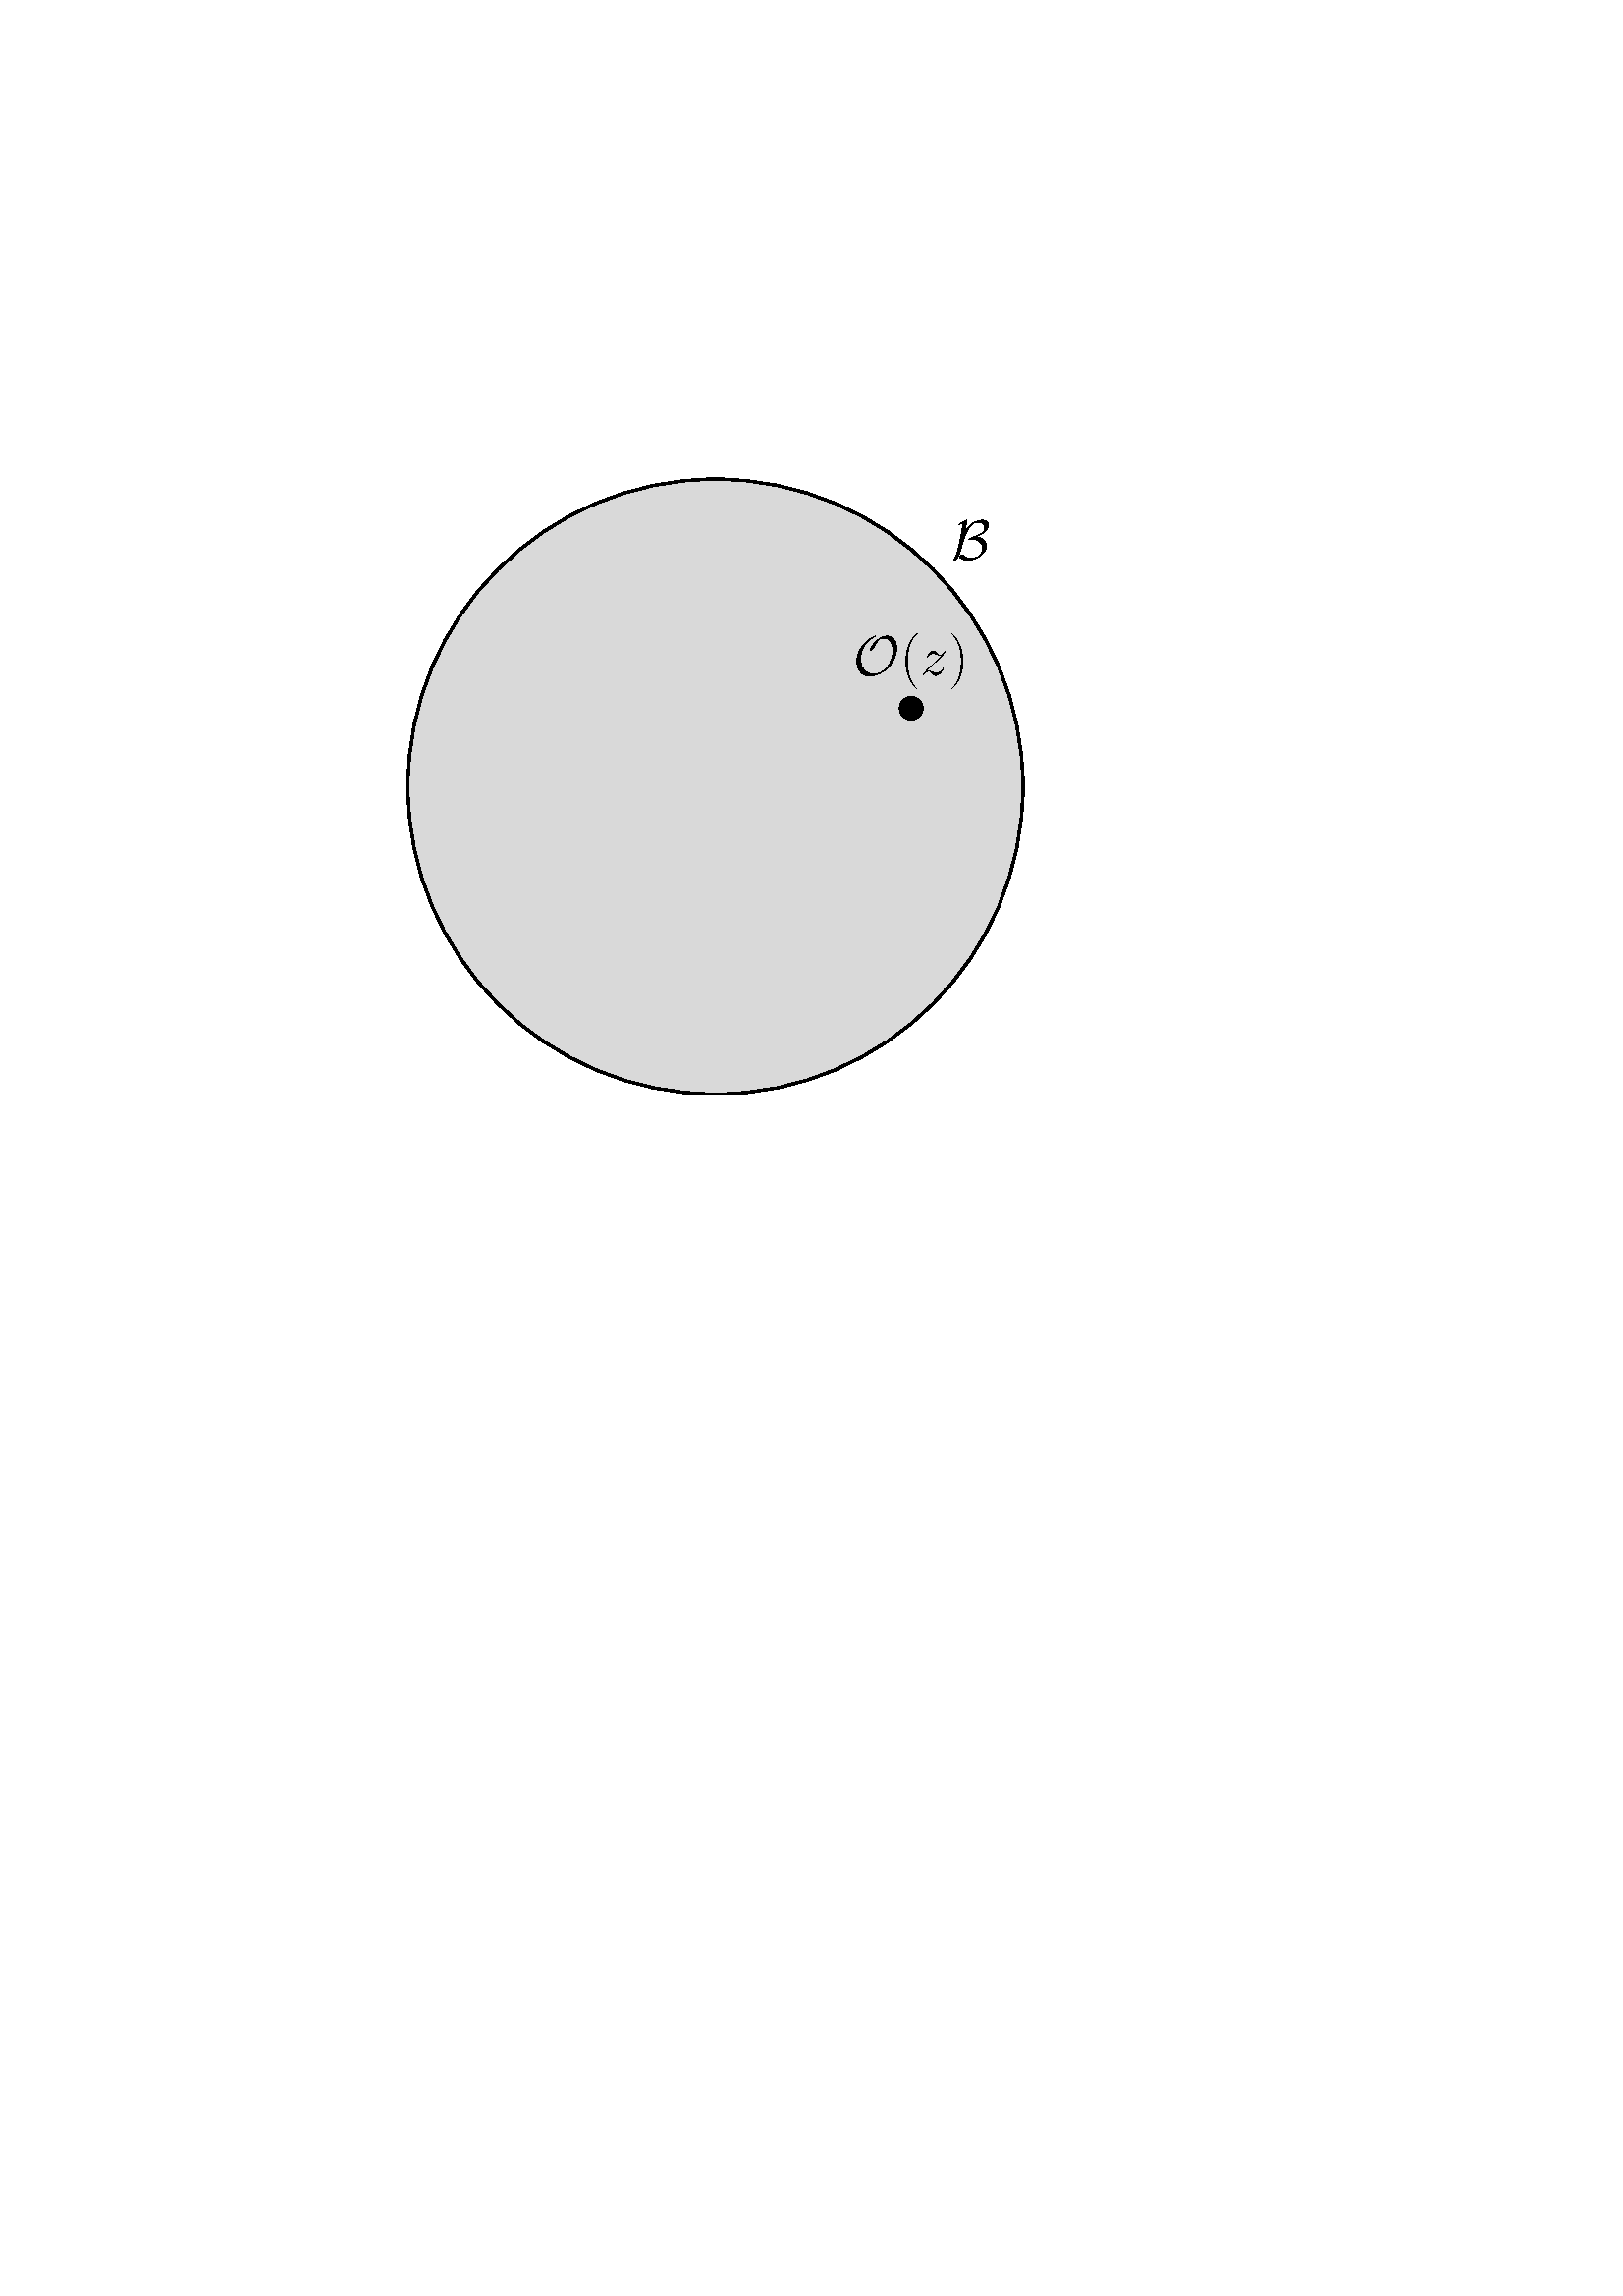
\includegraphics[width=0.75\linewidth]{figures/gla3-1.png}
\caption{ \medskip 在圆盘（阴影区域）内部一点 $z$ 处插入的局部算子 ${\EUO}(z)$，该圆盘的边界由膜 ${\cal B}$ 标记。当 $z$ 趋近圆盘边界时，${\EUO}(z)$ 可能趋于一个复常数。若对适当的算子 ${\EUO}_{H_\alpha}$ 这一点成立，我们就说 ${\cal B}$ 支撑在 Hitchin 纤维化的纤维 $\CMF$ 上。（原文 Fig.~3）}
\label{fig:trampo}
\end{figure}

由于零膜支撑在单个点上，它位于 Hitchin 纤维化的单根纤维 $\CMF_p$ 上。这根纤维由方程 $H_\alpha = h_\alpha$ 刻画，其中 $H_\alpha$ 是相互对易的哈密顿量，$h_\alpha$ 是复常数。在量子层面，我们说膜 ${\cal B}$ 支撑在纤维 ${\CMF}_p$ 上，如果当 $z$ 趋近由膜 ${\cal B}$ 标记的边界时，算子 ${\EUO}_{H_\alpha}(z)$ 趋于 $c$-数 $h_\alpha$（\trampo）。膜 ${\cal B}_p$ 当然具有这一性质。

现在我们考虑对偶运算 $S$。它把 $G$ 换成 Langlands 对偶群 $^L\negthinspace G$，从而把零膜 ${\cal B}_p$ 变成靶空间为 $\MH(^L\negthinspace G,C)$ 的 sigma 模型中的对偶膜 $\tilde{\cal B}_p$。回看表 2，我们看到，由于 ${\cal B}_p$ 是 $(B,B,B)$ 型膜，$\tilde {\cal B}_p$ 将是 $(B,A,A)$ 型膜，即在复结构 $I$ 中为 $B$-膜、在复结构 $J$ 与 $K$ 中为 $A$-膜。

变换 $S$ 给出映射 $\Xi:{\EUBB}\to {}^L\negthinspace{\EUBB}$，其中 ${\EUBB}$ 是 $G$ 的 Hitchin 纤维化的基，$^L\negthinspace{\EUBB}$ 是 $^L\negthinspace G$ 的相应基。具体地说，若点 $v\in {\EUBB}$ 由方程 $H_\alpha-h_\alpha=0$ 定义，而 $S$ 把 $H_{\alpha}$ 映到 $^LH_{\alpha}$，则 $\Xi(v)$ 由方程 $^LH_\alpha-h_\alpha=0$ 定义。如上所述，对单连通型 $G$，映射 $\Xi$ 是恒等映射。

把 $S$ 应用到 \trampo 的情形，我们观察到：若对膜 ${\cal B}$，算子 ${\EUO}_{H_\alpha}(z)$ 当 $z$ 趋近边界时趋于 $h_\alpha$，则对对偶膜 $\tilde {\cal B}$，对偶算子 ${\EUO}_{\tilde H_\alpha}(z)$ 在同一极限下同样趋于 $h_\alpha$。因此，若膜 ${\cal B}$ 支撑在 $G$ 的 Hitchin 纤维化的纤维 ${\CMF}$ 上，则其 $S$-对偶是支撑在 $^L\negthinspace G$ 的 Hitchin 纤维化的相应纤维 $\tilde {\CMF}=\Xi({\CMF})$ 上的膜 $\tilde {\cal B}$。

因此，$\tilde{\cal B}_p$ 是 $(B,A,A)$ 型膜，且支撑在对偶 Hitchin 纤维化的纤维 $\tilde {\CMF}$ 上。让我们聚焦于 $\tilde{\cal B}_p$ 为 $A$-膜的那些复结构 $J$ 与 $K$。一般地，空间 $X$ 中 $A$-膜的支撑至少是中间维数的。最熟悉的 $A$-膜支撑在中间维数的 Lagrangian 子流形上；也存在更奇异的余各向同性（coisotropic）$A$-膜，其支撑高于中间维数 \cite{ref80}。但中间维数是 $A$-膜支撑维数的下界。

然而，像 $\tilde {\cal B}_p$ 这样支撑在纤维 $\tilde {\CMF}$ 上的 $A$-膜，其支撑 {\it 至多} 是中间维数的。为调和这些约束，$\tilde{\cal B}_p$ 的支撑必须恰好是 $\tilde {\CMF}$。的确，如第~\ref{sec:hitchfib}~节所解释，$\tilde {\CMF}$ 在复结构 $I$ 中全纯，并且关于辛结构 $\omega_J$ 与 $\omega_K$ 是 Lagrangian 的。所以包在 $\tilde {\CMF}$ 上、并带有平坦酉 Chan-Paton 丛 ${\cal L}$ 的膜确实是 $(B,A,A)$ 型膜。

下面我们比较两边的模空间，只限于一边支撑在 ${\CMF}$ 上或另一边支撑在 $\tilde {\CMF}$ 上的膜。在这一限制下，${\cal B}_p$ 的模空间就是 ${\CMF}$ 的一份拷贝：$p$ 可以是 ${\CMF}$ 中任意点。

与此同时，对偶膜 $\tilde{\cal B}_p$ 的模空间是复环面 ${\EUJ}_{\tilde {\CMF}}$，它参数化 $\tilde {\CMF}$ 上秩为 1 的平坦 Chan-Paton 丛。（秩为 1，否则 $\tilde{\cal B}_p$ 的模空间维数将大于 ${\cal B}_p$ 的，$S$-对偶就不能成立。）${\EUJ}_{\tilde {\CMF}}$ 与 ${\CMF}$ 或 $\tilde {\CMF}$ 维数相同。显然，$S$-对偶在 ${\CMF}$ 与 ${\EUJ}_{\tilde {\CMF}}$ 之间建立同构。

当然，我们也可以反向进行。$\MH(^L\negthinspace G,C)$ 中位于 $\tilde {\CMF}$ 上一点处的零膜，同样被 $S$ 变换为 $\MH(G,C)$ 中包在 ${\CMF}$ 上、并带有平坦酉 Chan-Paton 丛的膜。所以 $S$-对偶同样在 $\tilde {\CMF}$ 与 ${\EUJ}_{\CMF}$（${\CMF}$ 上秩为 1 的平坦 Chan-Paton 丛的模空间）之间建立同构。

这幅图景就是环面纤维化之间的 SYZ 对偶。${\CMF}$ 参数化 $\tilde {\CMF}$ 上秩为 1 的平坦 Chan-Paton 丛，反之亦然。非正式地说，我们可以这样描述：运算 $S$ 通过映射 $\Xi:{\EUBB}\to{}^L\negthinspace{\EUBB}$（从一个 Hitchin 纤维化的基到对偶纤维化的基）连同在相应环面纤维上的 $T$-对偶来作用。这就是镜像对称通常的 SYZ 图景，只不过映射 $\Xi$ 通常被假定为平凡。

\begin{yizhu}[物理图像]
按：SYZ 图景把镜像对称拆成两部分：底空间之间一个通常取为恒等的映射，以及纤维环面之间的 $T$-对偶。对 Hitchin 纤维化，这个底映射恰好是四维 $S$-对偶在基上的经典作用 $\Xi$，对 simply-laced $G$ 取恒等；而纤维上的 $T$-对偶对应零膜到包在纤维上的膜的转换。这就是本节开头「在基上经典地作用、在纤维上通过 $T$-对偶作用」的精确含义。
\end{yizhu}

对酉群，$G$ 与 $^L\negthinspace G$ 的 Hitchin 纤维化的相应纤维互为对偶复环面，这一点已由 Hausel 与 Thaddeus \cite{ref21} 证明。对例外 Lie 群 $G_2$，Hitchin 最近建立了这一对偶 \cite{ref81}。Donagi 与 Pantev 用谱覆盖的抽象方法对任意半单 Lie 群分析了这一问题 \cite{ref82}。另见 Faltings 关于 $G$-丛的工作 \cite{ref83}。

在这一解释中，我们略去了关于该对偶的若干重要微妙之处。有些问题涉及 $G$ 的中心与基本群，在第~\ref{sec:centertop}~节有简要讨论。另一些问题涉及 $C$ 上自旋结构的作用，本文不分析。关于自旋结构的作用，以及中心与基本群的作用、酉群情形的对偶的更多细节，将另文发表 \cite{ref26}。

\subsection{$\MH$ 上的膜}

\label{sec:mhbranes}

我们已经遇到 $\MH$ 上膜的若干有趣例子——零膜与包在纤维上的膜。我们还会遇到其他例子。如同最初的例子，大多数重要的膜将关于三个复结构 $I$、$J$、$K$ 都具有超对称性质，这在理解它们的行为时非常有用。最令人感兴趣的膜保持有效二维 sigma 模型的一半超对称，而后者又具有底层规范场论的一半超对称。

例子包括 $(B,B,B)$-膜，即在每个复结构 $I,J,K$ 中都是 $B$-膜的膜，以及 $(B,A,A)$、$(A,B,A)$、$(A,A,B)$ 型膜，它们在一个复结构中为 $B$-型、在另外两个中为 $A$-型。我们已经看到 $S$ 把一个 $(B,B,B)$ 型膜与一个 $(B,A,A)$ 型膜互换。由表 2 还可看出，$S$ 把 $(A,B,A)$ 型膜映到同型的另一个膜，$(A,A,B)$ 型膜亦然。

给出这四种类型膜的例子并不困难；它们将是我们研究几何 Langlands 纲领时的重要膜。当然，更一般地，可以有这样的膜：它对复结构 $I,J,K$ 的任意线性组合为 $B$-型，而对两个正交的复结构为 $A$-型。\footnote{然而，不存在 $(B,B,A)$ 型膜。在复结构 $I$ 与 $J$ 中全纯的子簇自动在复结构 $K$ 中全纯。同样也不存在 $(A,A,A)$ 型膜。}

\begin{yizhu}[易错点]
按：膜类型的三个字母按复结构 $(I,J,K)$ 的次序排列，$B$/$A$ 分别指在该复结构中为 $B$-膜/$A$-膜。脚注的两个「不存在」来自超凯勒流形的复结构关系：在 $I,J$ 中全纯自动在 $K$ 中全纯，故没有 $(B,B,A)$；对 $A$-型也不可能有三个方向同时成立，故没有 $(A,A,A)$。
\end{yizhu}

我们已经研究过的零膜是最显然的 $(B,B,B)$ 型膜。$(B,B,B)$-膜的其他例子是填满空间的膜，其靶空间是整个 $\MH$，并带有在三个复结构中每一个都全纯的 Chan-Paton 向量丛。这类丛包括平凡丛，也包括其他例子，它们在几何 Langlands 纲领中的作用将另文讨论 \cite{ref26}。

一大类 $(B,A,A)$-膜的例子如下。设 $N$ 是 $\MH$ 在复结构 $I$ 中的复子流形，它关于全纯辛结构 $\Omega_I$、从而关于 $\omega_J$ 与 $\omega_K$ 是 Lagrangian 子流形。则支撑在 $N$ 上、带有平凡 Chan-Paton 丛的膜是 $(B,A,A)$-膜。我们已经遇到一个重要例子：$N$ 可以是 Hitchin 纤维化的纤维。另一个例子是，从复结构 $I$ 的角度，取 $N$ 为所有对 $(E,\varphi)$ 构成的空间，其中 $E$ 固定而 $\varphi$ 可变。从规范场论的观点，这意味着 $A_{\bar z}$ 在规范变换下固定，从而保证 $\Omega_I=(1/\pi)\int_C\,|d^2z|\,\Tr\,\delta\phi_z\wedge\delta A_{\bar z}$ 的消失。因此这给出 $(B,A,A)$ 型膜。

类似地，$(A,B,A)$ 与 $(A,A,B)$-膜的例子来自关于复结构 $J$ 或 $K$ 的复 Lagrangian 流形。复结构 $J$ 中复 Lagrangian 流形的一个简单例子，只需保持 ${\cal A}_{\bar z}=A_{\bar z}+ i\phi_{\bar z}$ 固定而让 ${\cal A}_z=A_z+i\phi_z$ 变化即可得到。这给出具有指定全纯结构的所有平坦 $G_{{\Bbb{C}}}$ 丛构成的族。类似地，通过指定 $A_{\bar z}-\phi_{\bar z}$ 并让 $A_z+\phi_z$ 变化，我们得到复结构 $K$ 中的复 Lagrangian 流形。在第~\ref{sec:abranes}~节，我们将把 $(A,B,A)$ 或 $(A,A,B)$ 型膜的更精细例子构造成「余各向同性膜」。
